\documentclass[tikz]{standalone}
\usepackage{pgfplots}
\pgfplotsset{compat=1.18}
\begin{document}
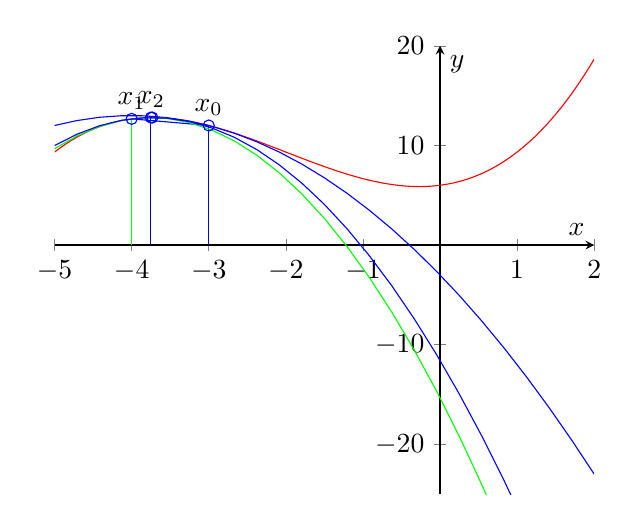
\begin{tikzpicture}
\begin{axis}[
    declare function={P(\x,\a,\b,\c)=\a*pow(\x,2)+\b*\x+\c;},
    axis lines=middle,
    % axis equal image,
    xlabel=$x$,
    ylabel=$y$,
    xmin=-5,xmax=2,
    ymin=-25,ymax=20,
    %xtick={2, 0 , 2, 4},
    %ytick={-5, 0, 5, 10},
    restrict x to domain=-5:2
    restrict y to domain=-10:10
    legend style={at={(axis cs:1,1)},anchor=nort west}
]
\addplot[domain=-5:2,samples=100,color=red]{x^3/3+2*x^2+x+6};
%\addlegendentry{$f(x)=1/3*x^3+2*x^2+x+6$}
\xdef\xold{-3}
\xdef\yold{12}
\xdef\a{0}
\xdef\b{0}
\xdef\b{0}
\foreach \k in {0,...,2}{
    \pgfmathsetmacro{\a}{\xold + 2}
    \pgfmathsetmacro{\b}{1-pow(\xold, 2)}
    \pgfmathsetmacro{\c}{pow(\xold, 3) / 3 + 6}
    \pgfmathsetmacro{\xnew}{\xold - ((pow(\xold, 2) + 4*\xold + 1) / (2*\xold+4))}
    \pgfmathsetmacro{\ynew}{pow(\xnew,3)/3+2*pow(\xnew, 2)+\xnew+6}
    % il punto sulla funzione
    \edef\punto{\noexpand\addplot[
        only marks,
        mark=circle,
        mark size=2pt,
        point meta=explicit symbolic,
        nodes near coords,
        ] coordinates {%
            (\xold,\yold) [$x_{\k}$]%
        };
    }
    \punto
      
    \ifodd\k
        % la parabola
        \addplot[domain=-5:2,color=green]{P(x, \a, \b, \c)};
        % il segmento verticale
        \addplot[mark=none,color=green] coordinates {(\xold,\yold) (\xold,0)};
    \else
        % il punto sulla funzione
        \addplot[mark=o,color=blue] coordinates {(\xold,\yold) (\xnew,\ynew)};
        % la parabola
        %\addplot[domain=-5:2,color=blue]{\a * x^2 + \b * x + \c};
        \addplot[domain=-5:2,color=blue]{P(x, \a, \b, \c)};
        % il segmento verticale
        \addplot[mark=none,color=blue] coordinates {(\xold,\yold) (\xold,0)};
    \fi
%    \addlegendentry{$k=\k$}
    \global\let\xold\xnew
    \global\let\yold\ynew
}
\end{axis}
\end{tikzpicture}
\end{document}